\documentclass[a4paper,11pt]{article}
\usepackage{graphicx}
\usepackage{enumerate}

\begin{document}

\begin{flushright}

\vspace{1.1cm}

{\bf\Huge Problem Set 3}

\rule{0.25\linewidth}{0.5pt}

\vspace{0.5cm}
%Put Authors
Justin Ely
\linebreak
\newline
%Put Author's affiliations
\footnotesize{605.411 Foundations of Computer Architecture \\}
\vspace{0.5cm}
% Date here below
20 September, 2016
\end{flushright}

\noindent\rule{\linewidth}{1.0pt}

%%%%%%%%%%%%%%%%%%%%%%%%%%%%%%%%%%%%%%%%%%%%%%%%%%%%%%%%%%

\section*{1)}
\begin{tabular}{| l | c | c | c | c | c | c | c | c |}
  \hline	
    1 & 2 & 3 & 4 & 5 & 6 & 7  \\  \hline \hline
    a & b & (ab)' & A'(3 )& B'(3) & ((4)(5))' & ((6)(6))'  \\  \hline \hline
    0 & 0 & 1 & 1 & 1 & 0 & 1  \\  \hline 
    1 & 0 & 1 & 0 & 1 & 1 & 0  \\  \hline 
    0 & 1 & 1 & 1 & 0 & 1 & 0  \\  \hline 
    1 & 1 & 0 & 1 & 1 & 0 & 1  \\  \hline 
\end{tabular} \\

\noindent  The result (last column) has the same truth table as a XNOR gate.

%%%%%%%%%%%%%%%%%%%%%%%%%%%%%%%%%%%%%%%%%%%%%%%%%%%%%%%%%%

\section*{2)} 


%%%%%%%%%%%%%%%%%%%%%%%%%%%%%%%%%%%%%%%%%%%%%%%%%%%%%%%%%%

\section*{3a)}
\begin{tabular}{| l | c | c | c | c | c | c | c | c |}
  \hline	
    1 & 2 & 3 & 4 & 5 & 6 & 7  \\  \hline \hline
    a & b & c & ab & bc & ac & (4) + (5) + (6)  \\  \hline \hline
    0 & 0 & 0 & 0 & 0 & 0 & 0  \\  \hline 
    0 & 0 & 1 & 0 & 0 & 0 & 0  \\  \hline 
    0 & 1 & 0 & 0 & 0 & 0 & 0  \\  \hline 
    0 & 1 & 1 & 0 & 1 & 0 & 1  \\  \hline 
    1 & 0 & 0 & 0 & 0 & 0 & 0  \\  \hline 
    1 & 0 & 1 & 0 & 0 & 1 & 1  \\  \hline 
    1 & 1 & 0 & 1 & 0 & 0 & 1  \\  \hline 
    1 & 1 & 1 & 1 & 1 & 1 & 1  \\  \hline 
\end{tabular} \\

\section*{3b)}
AB + BC + AC

%%%%%%%%%%%%%%%%%%%%%%%%%%%%%%%%%%%%%%%%%%%%%%%%%%%%%%%%%%

\section*{4)}
\begin{tabular}{| l | c | c | c | c | c | c | c | c |}
  \hline	
    1 & 2 & 3 & 4 & 5 & 6  \\  \hline \hline
    a & b & ab & a'b'& (3) + (4) & (5)'  \\  \hline \hline
    0 & 0 & 0 & 1 & 1 & 0   \\  \hline 
    1 & 0 & 0 & 0 & 0 & 1   \\  \hline 
    0 & 1 & 0 & 0 & 0 & 1   \\  \hline 
    1 & 1 & 1 & 0 & 1 & 0   \\  \hline 
\end{tabular} \\

\noindent This logic circuit can be replaced with a single XOR gate.

%%%%%%%%%%%%%%%%%%%%%%%%%%%%%%%%%%%%%%%%%%%%%%%%%%%%%%%%%%

\section*{5)}


%%%%%%%%%%%%%%%%%%%%%%%%%%%%%%%%%%%%%%%%%%%%%%%%%%%%%%%%%%

\section*{6)}

From problem 1, column 6 is the same output as an XOR gate, and has been constructed with only NAND gates.  Thus, the circuit
would look like that shown in the figure below.

\begin{figure}[h]
\caption{Circuit diagram for an XOR gate using only NAND gates.}
\centering
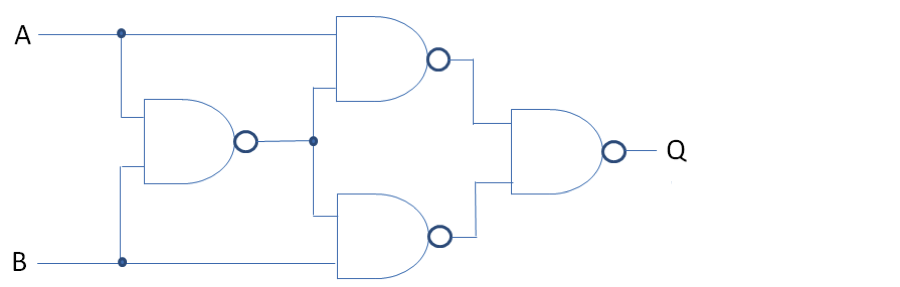
\includegraphics[width=1\textwidth]{p6_circuit.png}
\end{figure}

%%%%%%%%%%%%%%%%%%%%%%%%%%%%%%%%%%%%%%%%%%%%%%%%%%%%%%%%%%

\section*{7)}


%%%%%%%%%%%%%%%%%%%%%%%%%%%%%%%%%%%%%%%%%%%%%%%%%%%%%%%%%%

\section*{8)}


%%%%%%%%%%%%%%%%%%%%%%%%%%%%%%%%%%%%%%%%%%%%%%%%%%%%%%%%%%

\end{document}
